\chapter{Visual Scalability }
\label{chap:scalability}

This work studies how well these techniques scale to large data. To define the ability of visualizations to present large amounts of data we introduce the term \textit{visual scalability}.
Visual or perceptual scalability is defined as the capability of visualization tools in displaying large data sets in an effective manner  \cite{Eick2002}\label{effective}. In the context of time-oriented business data effective means the presentation of patterns to support the user tasks. To measure the visual scalability of different visualization techniques for time-oriented data we refer to the work of Eick  \cite{Eick2002}. He proposed to measure visual scalability by the database metrics of the data set and the visual characteristics of the visualization technique. \\*
\textbf{Database metrics}\label{databasemetrics} measures the \textit{size of the database} in bytes, the number of rows or the number of attributes at the level of the visualization tool. For multi-dimensional data the \textit{database metrics} are a combination of the number of rows and the attributes. \\*
\textbf{Visualization characteristics} describe the number of elements and attributes presented on the screen and measure how many distinct items a visualization technique can display. This number is measured on the visualization technique level.\\*
The combination of the database metrics and the visualization characteristics describes the scalability of a visualization tool. Furthermore, the tools scalability is influenced by more factors which will be discussed later (\ref{factors}).

\section{Visual Scalability of time-oriented techniques}\label{visualization}
The analysis of visualization techniques showed that time-oriented techniques are classified in only four of Keim's visualization classes: geometric, hierarchical, icon-based and pixel-oriented. In table \ref{table:vizScalability} we will name the corresponding techniques for multivariate time-oriented data. Subsequently, we will discuss the visualization characteristics for each class. 


\begin{table}[H]
	\centering
	\caption[Visualization Classes]{Visualization Classes}
	\label{table:vizScalability}
	\begin{tabu}{  | l | l | l |}
	\toprule
	Visualization Class & Technique & References\\
	\midrule
	    \multirow{8}*{Geometric} 
		& EventRiver        &  \cite{Luo2012}\\
		& Flocking Boids    &  \cite{Moere2004}\\
	    & Kiviat Tube       &  \cite{Tominski2005}\\
        & MultiComb         &  \cite{Tominski2004}\\
        & Multi-resolution CircleView &  \cite{Keim2005}\\
        & Parallel Glyphs   &  \cite{Fanea2005}\\
        & Temporal Star     &  \cite{Noirhomme-Fraiture2002}\\
        & TimeWheel         &  \cite{Tominski2004}\\ \hline
        \multicolumn{3}{|p{\linewidth}|}{
        The visualization characteristics of geometric projection techniques (GP-techniques) strongly depend on the mapping-function which regulates the projection of multi-dimensional data to the 2D screen  \cite{FerreiradeOliveira2003}. The mapping-function often includes data reduction techniques (see section \ref{analytical}).  When data reduction techniques are involved, this class of techniques is able to visualize large to huge data sets. This class will be described in detail (\ref{GP-Techniques}).} \\ \hline
        
		\multirow{3}*{Hierarchical} 
		& Pixel-Oriented Network Visualization  &  \cite{Stein2013}\\
		& Software Evolution Analysis   &  \cite{Gall1999}\\
		& Timeline Trees                &  \cite{Burch2008}\\ \hline
		\multicolumn{3}{|p{\linewidth}|}{We analyzed three hierarchical visualization techniques. Timeline Trees included aggregation techniques by collapsing nodes. With collapsed nodes the technique can display large to huge amounts of data. Pixel-oriented Networks use clustering and thus, \todo{Begrüdung für Skalierbarkeit einfügen}} \\ \hline
        \multirow{5}*{Icon-based}
        & Gravi++       & \cite{Hinum2005}\\
        & InfoBUG       & \cite{Chuah1998}\\
        & PeopleGarden  & \cite{Xiong1999}\\
        & Spiral Graph  & \cite{Weber2001}\\
        & VIE-VISU      & \cite{Horn2001}\\ \hline
        \multicolumn{3}{|p{\linewidth}|}{
        As every data item requires one icon icon-based techniques can show less data items than the number of pixels on the screen. When showing large data icon-based techniques face the challenge of clutter and occlusion \cite{Borgo2013}. Thus, icon-based techniques can only display small- to medium-sized data sets.}\\ \hline
        \multirow{12}*{Pixel-oriented}
        & 3D ThemeRiver &  \cite{Imrich2002}\\
        & Braided Graph &  \cite{Javed2010}\\
        & CircleView    &  \cite{Keim2005}\\
        & Data Tube Technique &  \cite{Ankerst2001}\\
        & history flow  &  \cite{Viegas2004}\\
        & Kaleidomaps   &  \cite{Bale2007}\\
        & Pixel-Oriented Network Visualization  &  \cite{Stein2013}\\
        & Recursive Pattern &  \cite{Keim1995}\\
        & Spiral Display    &  \cite{Carlis1998}\\
        & Stacked Graphs    &  \cite{Byron2008}\\
        & ThemeRiver        &  \cite{Havre2000}\\
        & Time Curves       &  \cite{Bach2016}\\
        & TimeRider         &  \cite{Rind2011}\\ \hline
        \multicolumn{3}{|p{\linewidth}|}{
        Since only one pixel per data item is used this class can maximize the used screen space. Let $M$ be the monitor resolution with the screen-width $w$ and the screen-height $h$, $P$ the number of pixels in $M$ and $D$ the maximum of data which can be displayed at once. In pixel-oriented techniques  \begin{math}
        D = w*h
        \end{math}
        which shows that pixel-oriented techniques can display large, but not huge data.}
        \\ \hline
	\bottomrule
	\end{tabu}
\end{table}


Most of the existing visualization techniques nowadays still are not appropriate in visualizing huge data as summarized in table \ref{table:vizScalability}. Pixel-based visualizations represent each data item by one pixel and thus, are limited to two million pixels. Even new visualization techniques which where developed to visualize "very large" data sets follow the pixel-oriented approach  \cite{Keim1995, Keim1996}. Icon-based visualizations display one data item per icon and thus can display even less data than pixel-oriented visualizaton techniques. The most promising techniques are hierarchical and geometric-projective techniques as they combine aggregation or abstraction with visualization. Their scalability depends on the mapping-function. 
One interesting extension of pixel-oriented techniques is the \textit{multi-resolution} approach  \cite{Keim2005}. The idea is to show more relevant data items at a pixel-based level and less relevant data items in an aggregated way. The technique \textit{multi-resolution CircleView} shows recent data at full resolution in the middle of the circle and places previous-year-data  at the outer circle. With multi-resolution it is possible to extent the pixel-limit from $w*h$ to larger data sets. 

\begin{table}[H]
	\centering
	\caption[Scalability of Visualization Classes]{Scalability of Visualization Classes}
	\label{table:vizScalability}
	\begin{tabu}{ l | c }
	\toprule
	Visualization Class & Scalability\\
	\midrule
	Geometric &  \cellcolor{green!25 } > 2 mio. pixel\\
	Hierarchical & \cellcolor{green!25} > 2 mio. pixel \\
	Icon-based & \cellcolor{red!25} $\leq$ 1 mio. pixel \\
	Pixel-oriented & \cellcolor{yellow!25} $\leq$ 2 mio. pixel \\	
	\bottomrule
	\end{tabu}
\end{table}





%Aspects of Scalability:
% Wie viele Datenpunkte sind notwendig, um Pattern darzustellen? -> data 
% Interaction Techniques
% Downsampling -> Analytical Methods
\iffalse
 The challenges of large-scale data for ADV are \textit{scalability} and \textit{dynamics}  \cite{Wang2015}. With its volume the challenges for large-scale data are also challenges for Big Data defined as high volume, high velocity, high veracity and high variety data sets  \cite{Wang2015}. In this work we concentrate on the scalability challenge for visualization techniques. The challenge is in finding appropriate techniques  \cite{Aigner2008,Keim2005} which scale to large amount of data.
 
\fi

\subsubsection{Visualization characteristics of GP-Techniques} \label{GP-Techniques}
Geometric-projective visualizations seems to be the most scalable visualization technique depending on the mapping function. For this reason we will explore techniques in the geometric-projective class in detail and discuss their scalability.


Furthermore, we suggest to divide GP-techniques into \textit{radial} and \textit{non-radial} visualizations  \cite{Diehl2010} (compare table \ref{table:radialTable}) as our  analysis has shown that a large part of GP-techniques is based on a radial layout. Radial GP-techniques share common properties such as the maximum number of attributes which is set to 10-20 attributes  \cite{Diehl2010}.\\*


\begin{table}[H]
	\centering
	\caption[Radial and non-radial GP-techniques]{Radial and non-radial GP-techniques}
	\label{table:radialTable}
	\begin{tabu}{lcc}
	\toprule
	GP-Technique & radial & non-radial \\
	\midrule
	Flocking Boids &  & x \\
	Kiviat Tube & x &  \\
	MultiComb & x &  \\
	Multi-resolution CircleView & x &  \\
	Parallel Glyphs & x &  \\
    Temporal Star & x &  \\
	TimeWheel & x & \\
	\bottomrule
	\end{tabu}
\end{table}

As discussed in \ref{chap:scalability} the scalability of visualizations is measured by the number of distinct items. Distinct items are calculated with the maximum number of data items * the maximum number of attributes. 

\textbf{Flocking Boids} (figure \ref{fig:flockingboids}) simulate the evolution of data items in 3D. Thus, data objects are represented by a colored, curved line with changing transparency called \textit{boid}.  A data object is an aggregation of same data items, e.g. one boid is one stock market company. A boid calculates the average of multiple data attributes and uses behavior rules to simulate the development of a data object. The rules define the position of data item over time and its velocity. Thereby, time is represented by animation and boids correspond to distinct items on the screen. Thus, the maximum measured number of used boids defines the scalability. Flocking Boids were able to handle 500 boids at a time. Thus the scalability of Flocking Boids is 500 which is low compared to pixel-oriented techniques(two million items)  \cite{Moere2004}.
Analytical Methods such as clustering or subset selection are outsourced to database algorithms and interaction techniques are not implemented but could be extended \cite{Moere2004}. 
\begin{figure}[H]
    \centering
        \scalebox{.3}{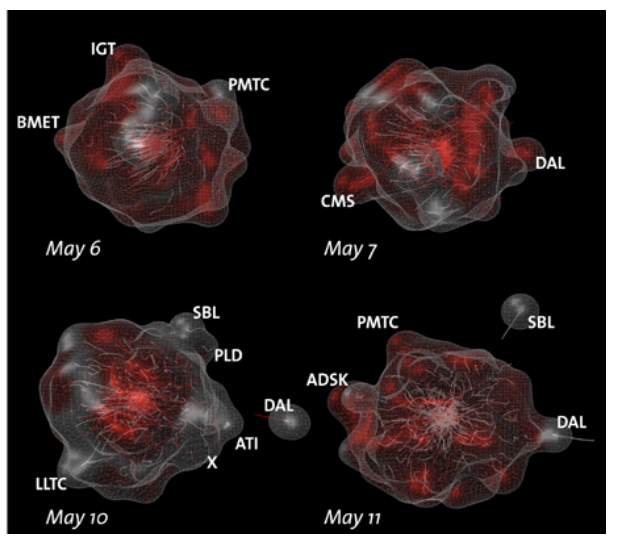
\includegraphics{src/images/FlockingBoids}}
    \caption{Flocking Boids. From  \cite{Aigner2011}.}
    \label{fig:flockingboids}
\end{figure}
\\*
\textbf{Kiviat Tube} (figure \ref{fig:kiviattube}) is an unfolded Radar Chart along the z axis in 3D. Several Radar Charts are stacked behind each other along the time (z) axis and form a tube. Thus, variables are mapped on radial aligned planes and can be compared. Interaction such as changing the planes positions and navigating through time enables the user to compare different variables over time.\\*
The number of attributes is limited to approximately 10-20 attributes as the radial layout limits the number of variables. As the Kiviat Tube is a 3D representation the tube is projected to the 2D screen. Let $w$ be the window width. Then, the maximum number of data items is $\leq w$ as the technique does not include any aggregation. The scalability is $20*w\approx 20.000$.
\begin{figure}[H]
    \centering
        \scalebox{.3}{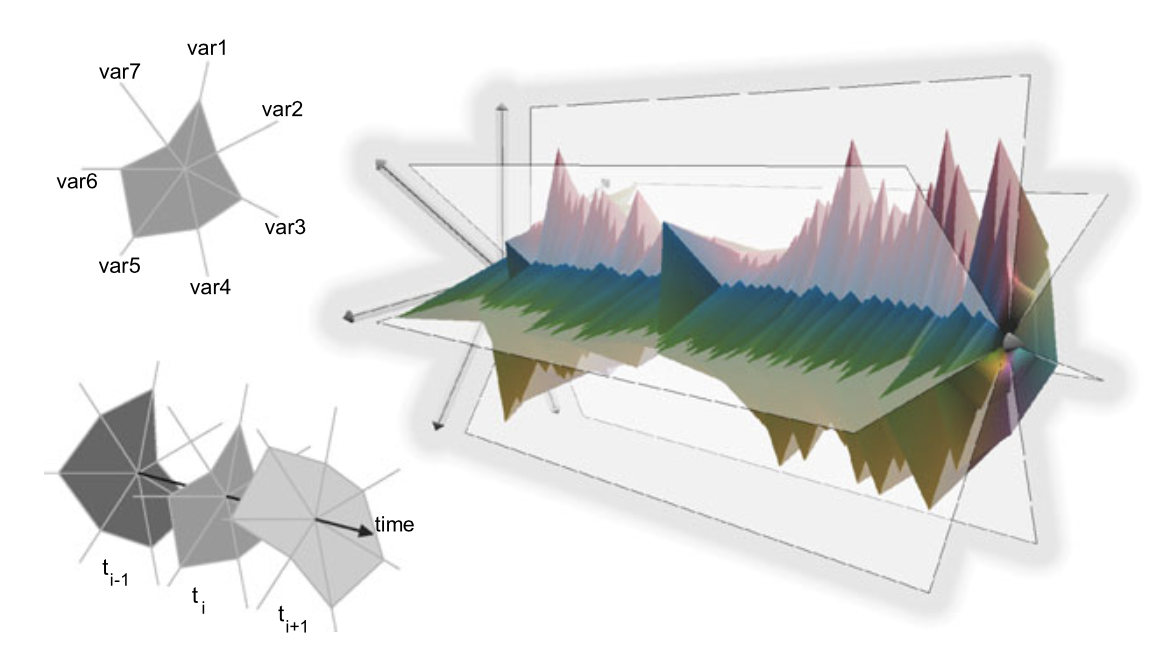
\includegraphics{src/images/KiviatTube}}
    \caption{Kivit Tube. From  \cite{Aigner2011}.}
    \label{fig:kiviattube}
\end{figure}
\\*
In \textbf{MultiComb} (figure \ref{fig:multicomb}) \textit{k} time series plots are mapped on a circle in two possible ways. One way is to position the plots along the circumference. Or the plots are mapped perpendicular to the circumference. In this version the plot resembles a star.  The MultiComb is radial. Let $h$ be the window height, then the maximum number of data items in version two is $< \frac{h}{2}$ and the scalability $20*< \frac{h}{2} \approx 10.000$
\begin{figure}[H]
    \centering
        \scalebox{.3}{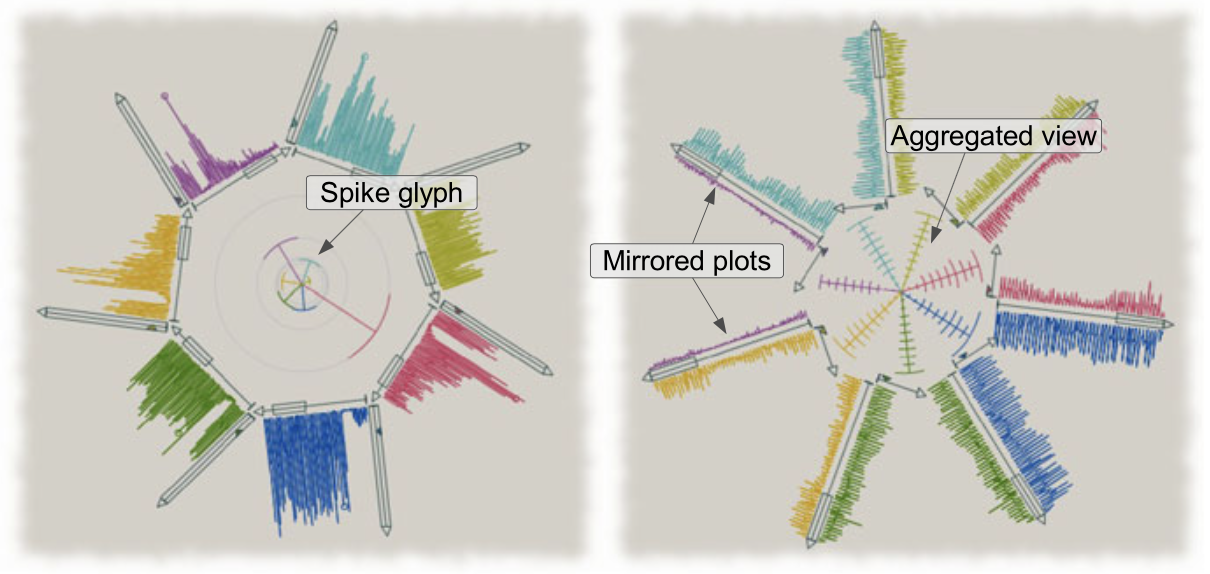
\includegraphics{src/images/MultiComb1,2}}
    \caption{Multi Comb. From  \cite{Luo2012}.}
    \label{fig:multicomb}
\end{figure}
\\*
\textbf{Multi-resolution CircleView} (figure \ref{fig:multiresolutioncircleview}) enhances the CircleView technique. Instead of mapping each value to one pixel, data items are aggregated. More recent items are placed in the middle of the circle. These items are represented by one pixel each. Less relevant items are aggregated and placed at the outer part of the circle. These items are usually from a preceding point of time. As Multi-resolution CircleView uses aggregation the maximum number of data items is $> 2mio.$ pixels which makes multi-resolution circle view to a scalable visualization.
\begin{figure}[H]
    \centering
        \scalebox{.3}{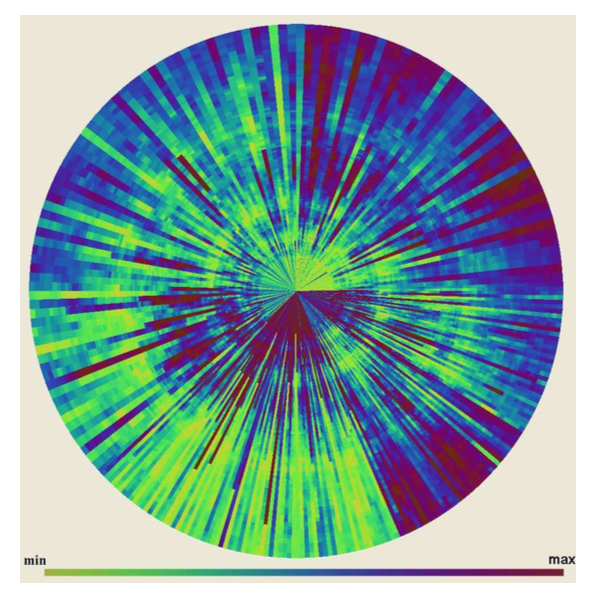
\includegraphics{src/images/MultiResolutionCircleView}}
    \caption{Multi-resolution CircleView. From  \cite{Keim2005}.}
    \label{fig:multiresolutioncircleview}
\end{figure}
\\*
\textbf{Parallel Glyphs} (figure \ref{fig:parallelglyphs}) pair Parallel Coordinates with Star Glyphs. While similar to Parallel Coordinates each data item is represented by a polyline which connects the vertical axis (attributes) the attribute axis are radially unfolded in 3D and show the data value of the data item over time. Thus, each data value over time is represented by a star glyph. The visualization can be expanded by connection lines over star glyphs. Parallel Glyphs provide brushing of polylines, filtering, axis reordering, rotating in three directions, transparency support if the glyphs overlap each other, focus+context presentation through magnification lenses. Through the extension of 2D to 3D parallel glyphs are able to display more data rows than parallel coordinates (PC). PC had the problem of clutter while displaying 15.000 data items on a gray-scale  \cite{Keim2000Tut}. Yet, as the maximum number of data items is below one mio. data points parallel glyphs are no scalable visualization technique. 

\begin{figure}[H]
    \centering
        \scalebox{.3}{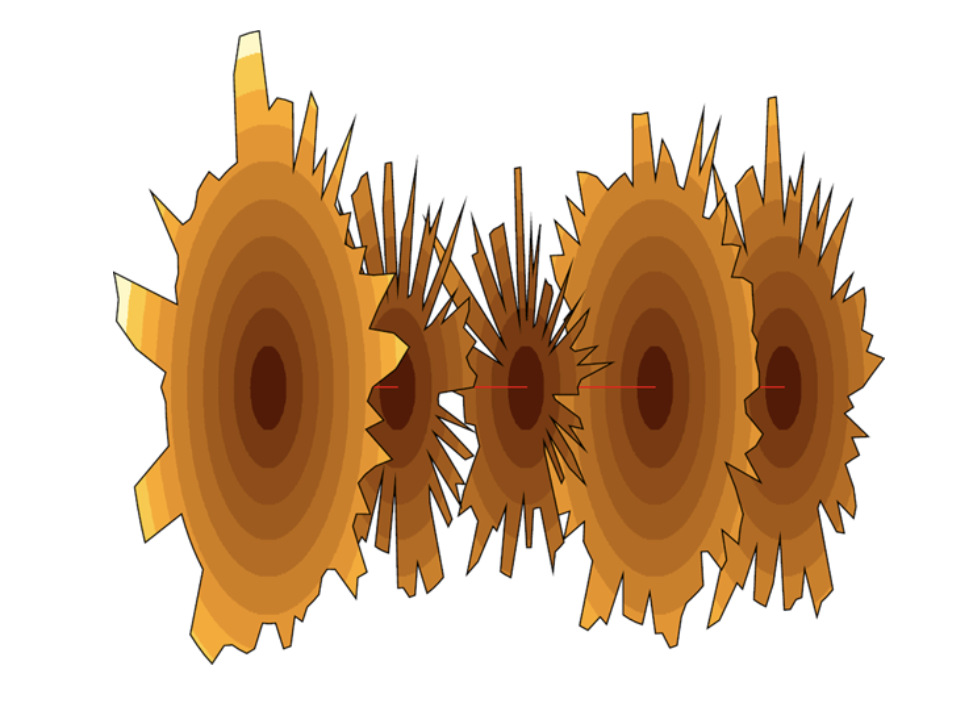
\includegraphics{src/images/ParallelGlyphs}}
    \caption{Parallel Glyphs. From  \cite{Aigner2011}.}
    \label{fig:parallelglyphs}
\end{figure}\\*

\textbf{Temporal Star} (figure \ref{fig:temporalstar}) aligns multiple attributes in a star-like manner around the centre. Each star is one point of time. The time axis connects several stars to a 3D-object. Temporal star uses so called \textit{symbolic objects} to display aggregated data. This way temporal star is designed to show large data sets. 
\begin{figure}[H]
    \centering
        \scalebox{.3}{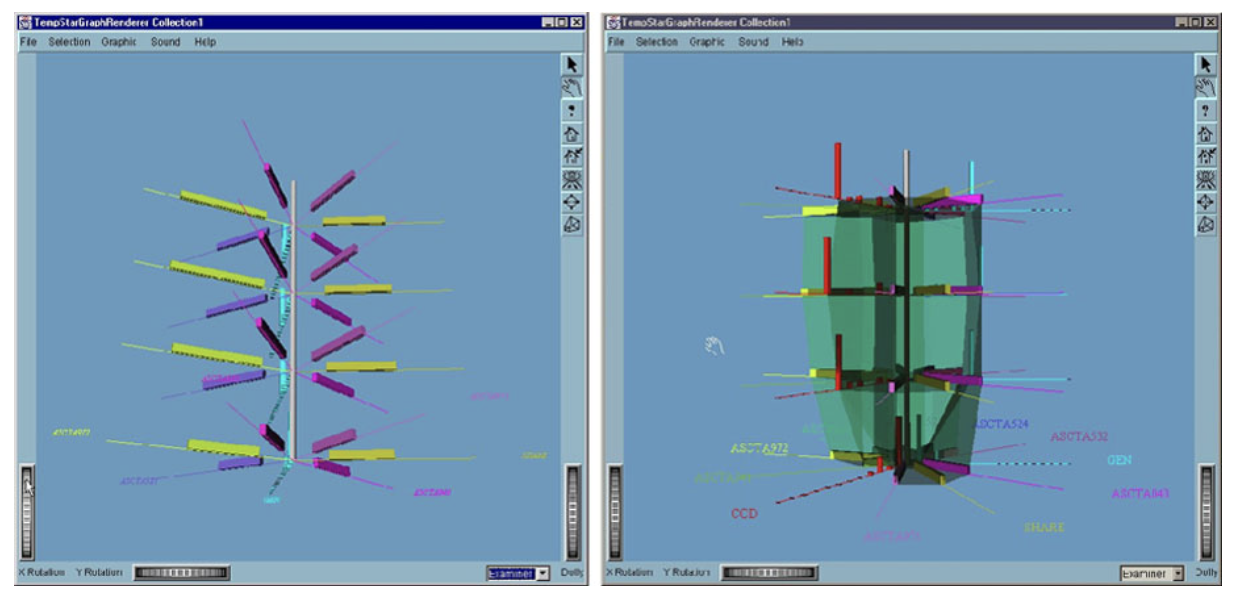
\includegraphics{src/images/TemporalStar}}
    \caption{Temporal Star. From  \cite{Aigner2011}.}
    \label{fig:temporalstar}
\end{figure}\\*

\textbf{TimeWheel} (figure \ref{fig:timewheel}) is a 2D technique. Similar to variation one of \textit{MultiComb} attribute axis are positioned along the circle circumference. In the centre of the circle the time axis is placed. Let $a$ be the pixel width of this axis and $a < w$. Similar to MultiComb Time Wheel does not include aggregation and thus the maximum number of data items is limited to $a$. Thus, the scalability is $20* <w \approx 10.000$.
\begin{figure}[H]
    \centering
        \scalebox{.3}{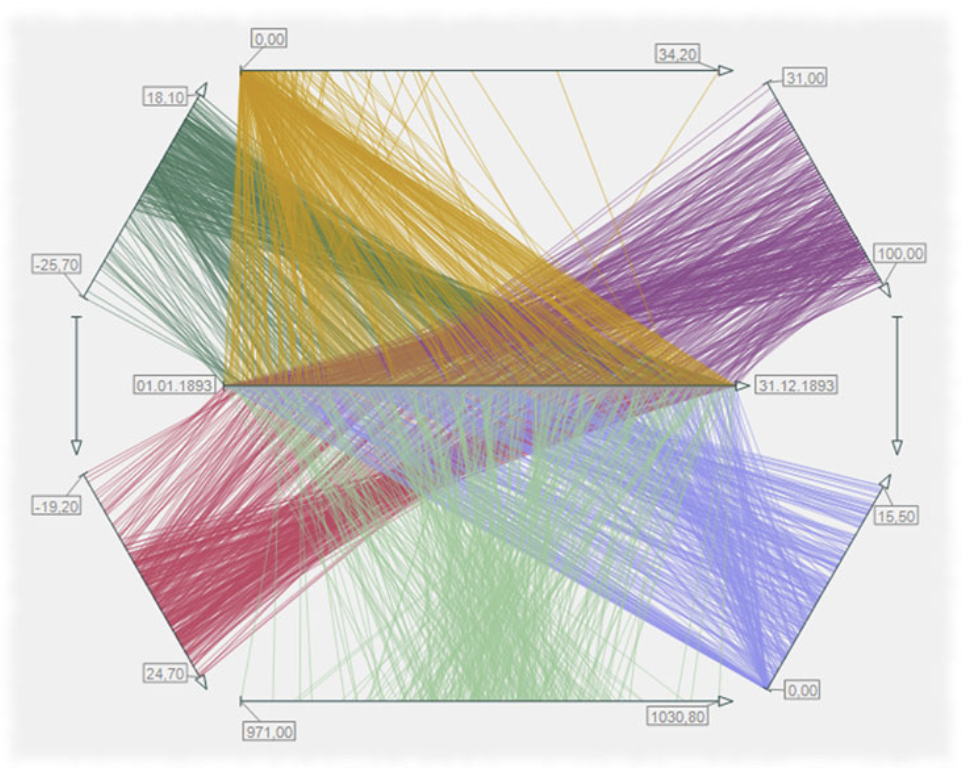
\includegraphics{src/images/TimeWheel}}
    \caption{Time Wheel. From  \cite{Aigner2011}.}
    \label{fig:timewheel}
\end{figure}\\*

\begin{table}[H]
	\centering
	\caption[Scalability of GP-Techniques]{Scalability of GP-Techniques}
	\label{table:GPscalability}
	\begin{tabu}{lcc}
	\toprule
	GP-Technique & scalability \\
	\midrule
	Flocking Boids & \cellcolor{red!25 }500* \\
	Kiviat Tube & \cellcolor{red!25 }20.000 \\
	MultiComb & \cellcolor{red!25 }10.000 \\
	Multi-resolution CircleView & \cellcolor{green!25 }$>$ 2mio.\\
	Parallel Glyphs &  \cellcolor{yellow!25 }15.000 - $>$ 1mio.\\
    Temporal Star &  \cellcolor{green!25 }$>$ 2mio.\\
	TimeWheel & \cellcolor{red!25 }10.000\\
	\bottomrule
	\end{tabu}
\end{table}

Geometric-projective techniques are limited in the maximum numbers of items. Out of the four visualization classes \textit{multi-resolution CircleView, Temporal Star and hierarchical techniques} are appropriate to visualize large amounts of data as shown in table \ref{table:GPscalability}. 
% TCS: Optimum for ADV 
In summary, visualization tools should integrate advanced data visualization (ADV) to visualize time-oriented multivariate data. In our understanding ADV is a visualization technique which is able to scale to large and huge amounts of data. \\*
%\textit{Aigner et. al} classify Parallel Coordinates as standard visualizations \cite{Aigner2011} whereas \textit{Keim et. al.}  \cite{Keim} are talking about Parallel Coordinates as a novel technique. This discussion of course is determined by the time epoche. The longer a visualization technique is known the more it is counted as a standard visualization technique. 

However, only few techniques are able to represent billions of data. In the end, most of them are limited through the 2D-screen. Factors which enhance the scalability are \textit{advanced visual metaphors}, \textit{interaction techniques} and \textit{data reduction}. 



\section{More Factors} \label{factors}
Moreover, besides the database metrics and the visualization characteristics visual scalability is influenced by six factors \cite{Eick2002}: 
\begin{itemize}
    \item Monitor Resolution 
    \item Human Perception \cite{Keim2005,Deering1998}
    \item Visual Metaphors
    \item Interactivity
    \item Data Reduction
\end{itemize}

\section{Monitor Resolution}\label{resolution}
Even though large wall-sized screens have been developed nowadays monitors with a display width of 50 cm are used in business. Sometimes, -depending on the department- two or three monitors are combined for a larger wall. Thus, the maximum number of pixels which can be used at the workspace ranges from 786.432 (1024x768) to 6.912.000 (three monitors à 1920x1200).
Concluding, the available amount of data in a data set exceeds the maximal number of screen pixels by far. But, besides the available monitor resolution another limiting factor is the perceivable number of pixels by the human perception.

\section{Human Perception} \label{perception}
% What can humans perceive? How many pixels? 
The brain is limited in perceiving pixels on the screen as well as patterns created by visualizations. Since space in brain is represented different from the screen the term computer monitor pixels requires a brain equivalent for screen pixels. We call them brain pixels. According to  \cite{Ware2012a} brain pixels are nearly represented by ganglion cells. Ganglion cells are neurons which send information to the cortex. In the fovea one ganglion cell cares about one single cone. In the periphery one ganglion cell handles thousand rods and cones. Thus, the brain pixel resolution in the fovea is much higher than in the periphery. The brain aggregates pixels and adheres multi-resolution. 
To model how many data items are perceived by the human brain it is important to make the following distinction: 
\\*
\textit{TBP = total amount of brain pixels which is stimulated by the screen pixels}\\*
and unique stimulated brain pixels: \textit{USBP = TBP - redundant brain pixels}.\\*
USBP are the number of pixel who determines the human perception of data items. A measure of display efficiency (DE) is the ratio of USBP and screen pixels(SP): \textit{DE = USBP/ SP}.

Figure \ref{fig:DE} shows that a monitor larger than 40cm wide are not increasing the display efficiency anymore. For large data sets this allows the conclusion that the perception of large data has a limit in the human perception. The current monitor size (which approximately is  40-50cm) is sufficient to respond to the number of USBP.

\begin{figure}[H]
    \centering
    \scalebox{.3}{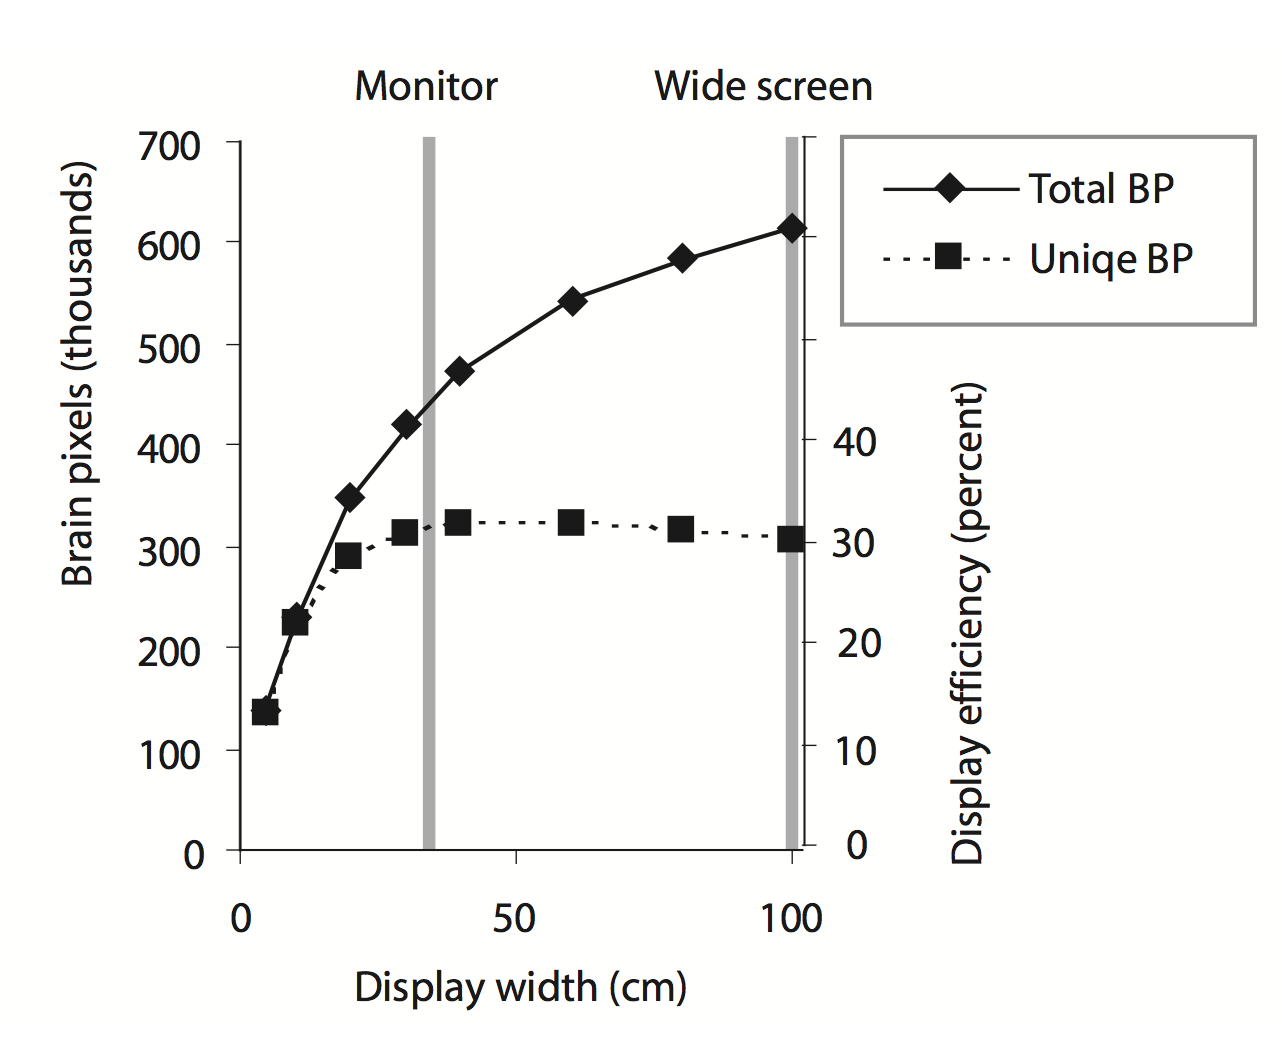
\includegraphics{src/images/DE}}
    \caption{Simulation of display efficiency by exposing the brain to a 1 mio. pixel screen. From  \cite{Ware2012a}.}
    \label{fig:DE}
\end{figure}

Talking of TBP  the human visual system is able to perceive 15mio pixels per eye  \cite{Deering1998}. Assuming that the amount of perceivable pixels for two eyes is larger than 15mio pixels but smaller than 30mio pixels due to the overlap of the field of view the max. amount of perceivable pixels (pp) is:
\begin{math}
15 mio. \leq pp < 30 mio.
\end{math}

Nevertheless, the important question is not the amount of perceivable pixels but whether the data structure, patterns, trends and further information in the data can be perceived as the human brain is a pattern detection machine  \cite{Ware2012a}. If we consider the brains ability to detect patterns aggregation methods for visualizations are not only tolerated but moreover recommended. Moreover, the main concern for visualization techniques should be the perception of patterns: trend, outliers, clusters. 
\par
In conclusion, human perception shows that visual scalability of techniques and monitor resolution are not important. The interesting question is whether tools integrate aggregation methods to outline patterns. \label{pattern}
Aggregation methods can either aggregate data inside the data set or inside the visualization. Examples for data set aggregation are calculated dimensions which joins multiple dimensions into a new one. Examples for visualization aggregation are clustered markers. The data set aggregation is discussed in section \ref{analytical} and visualization aggregation in section \ref{advancedmetaphor}.

\section{Analytical Techniques}\label{analytical}
Comparing the visualization techniques in \ref{vis} only few techniques scaled beyond two million pixels. Thus, the need for data reduction becomes obvious. In the literature \textit{data abstraction and aggregation} are well know techniques for data reduction  \cite{FerreiradeOliveira2003,Aigner2011, Keim2005}. There exist two ways to data reduction: to reduce data horizontally or vertically. 
Vertical data reduction describes the process of removing data rows (figure \ref{fig:vertical}) whereas horizontal data reduction (figure \ref{fig:horizontal}) is used for dimensionality reduction.

% \begin{figure}[H]
%     \centering
%         \scalebox{.1}{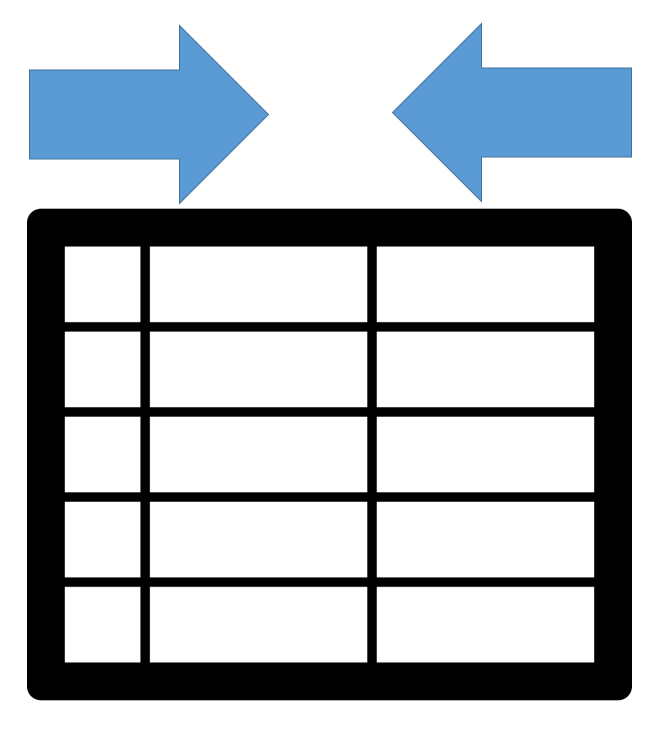
\includegraphics{src/images/dimreduce}}
%     \caption{Horizontal Data Reduction}
%     \label{fig:horizontal}
% \end{figure}

% \begin{figure}[H]
%     \centering
%         \scalebox{.1}{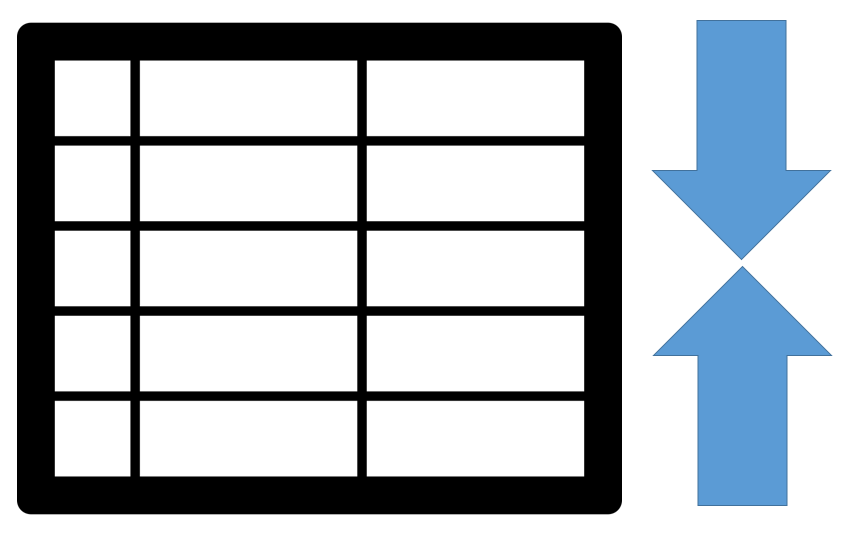
\includegraphics{src/images/aggregation}}
%     \caption{Vertical Data Reduction}
%     \label{fig:vertical}
% \end{figure}

\begin{figure}[H]
 \centering
        \subfloat[Horizontal Data Reduction]{\label{fig:horizontal}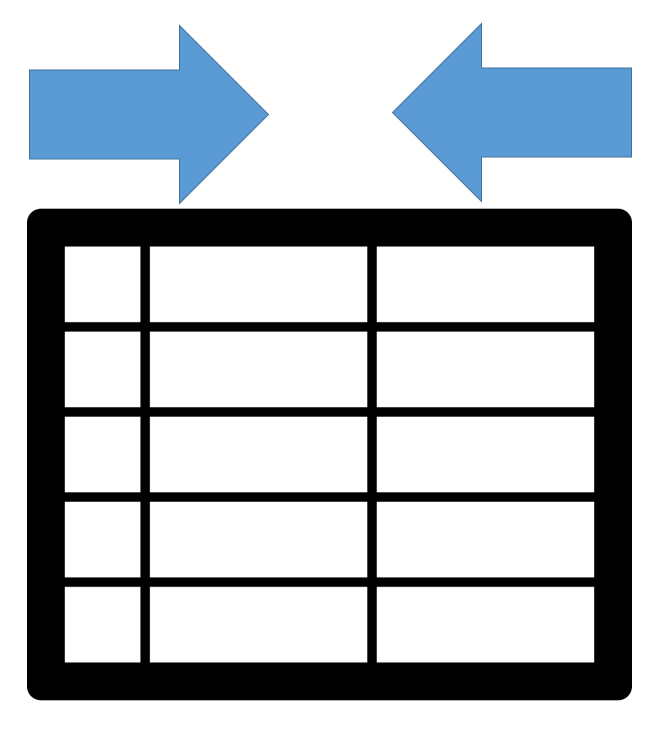
\includegraphics[width = 0.3\textwidth]{src/images/dimreduce}}
\qquad
\qquad

        \subfloat[Vertical Data Reduction]{\label{fig:vertical}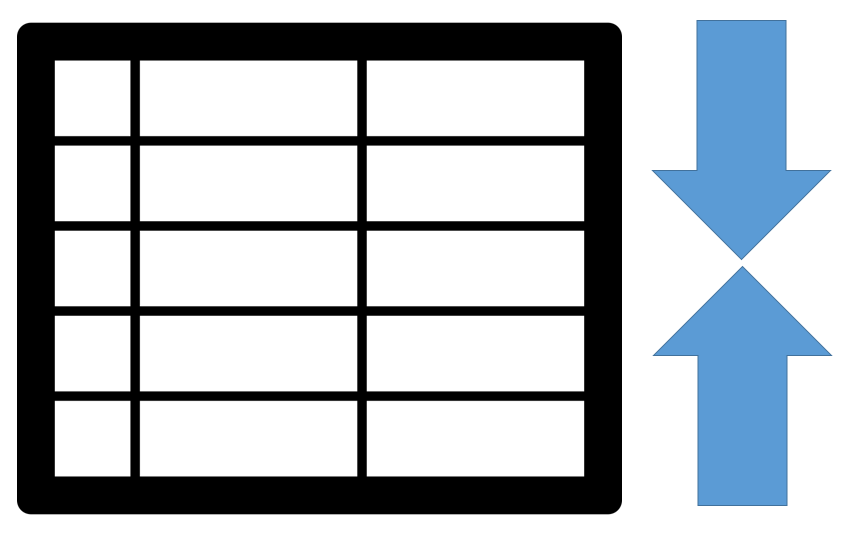
\includegraphics[width = 0.39\textwidth]{src/images/aggregation}}
\end{figure}

\subsection{Vertical Data Reduction}
One way to decrease the size of large or huge data sets is to remove data rows. This section lists several data removal techniques. 
%One important issue for every technique is the question which data to keep and which data to remove. The disadvantage of data reduction is the information loss.
\textbf{Sampling \& Filtering: }\label{sampling}\label{filtering}
Sampling describes a strategy to reduce data by creating a subset of the original data. Thereby, sampling is scalable, reduces clutter, preserves information of the kept data as well as patterns and trends \cite{PiringerHarald2011}. Still, sampling may eliminate outliers or single data items and does not provide any guarantee to avoid visual overlap. \\*
Filtering is a method to reduce data by some specific criteria. In visualization filtering often is based on user input such as dynamic query sliders in the frontend. In the backend filtering can also applied to define data extracts. In both cases filtering can support the user in excluding task-irrelevant data portions and unlike sampling filtering may be appropriate to detect outliers. However, as filtering is based on the exclusion of irrelevant attributes it does not guarantee a specific target size of the data set. In some cases the target size might still be too large. Moreover, filtering also does not secure the discrimination of distinct data items  \cite{PiringerHarald2011}.\\*
\textbf{Aggregation: }\label{aggregation}
Aggregation describes the process of grouping similar data items together. Hierarchical aggregation builds aggregated data items by forming a tree structure and collapsing the children of a tree  \cite{Elmqvist2010}. Binned aggregation divides data into adjacent bins and combines them for aggregation  \cite{Liu2013}. Pixel-aware aggregation clusters pixels according to their screen coordinates  \cite{Li2016}. M4 aggregation compresses time series data into a set of equidistant time spans  \cite{Jugel2014}.
As time-oriented data has specific characteristics analytical methods have to consider these peculiarities. One way to reduce data size with respect to the time-specific characteristics is temporal aggregation. Hereby, data is aggregated according to the time unit (day, month, year) in temporal hierarchy levels. Examples for temporal aggregation are hierarchical axis  \cite{Chung2014} which enable to navigate in time. 
\\*
\textbf{Temporal Data Abstraction: }\label{temporalabstraction}
Temporal Data Abstraction  \cite{Aigner2011} reduces the number of data rows by focusing on relevant concepts, patterns, shapes over time and neglecting irrelevant details. Clusters and summery statistics  \cite{PiringerHarald2011} are typical examples for data abstraction. In the context of time-oriented data  However, the authors found a trade-off between abstraction and accuracy: with low abstraction and a high accuracy there exists the problem of cluttering. 
One way to implement temporal data abstraction is to use natural language processing in visualization tools. The tool \textit{Answerrocket} implemented an NLP-Approach connected with visualization. Another way to achieve data abstraction are unsupervised machine learning methods, such as clustering.
Clustering as defined in the user tasks \ref{tasks} as \textbf{T2} has the advantage of reducing visual clutter by displaying the natural groups of the data instead of every single data item. It also preserves pattern and outlier if the similarity measure is appropriate.\\*
Temporal Data Abstraction in tools can be implemented by any method which keeps the characteristic shape and removes data points. \\*

Other ways to reduce data vertically are binning and pivoting. We will not explain them here in detail as they treat continuous and hierarchical data sets which are beyond our scope. 

\subsection{Horizontal Data Reduction}
Besides data removal data size can be reduced by decreasing data dimensionality. Since business data often is multi-dimensional but visualization techniques are limited in the number of attributes dimensionality reduction is a way to process data sets in a way that they can be displayed by visualization techniques. 
\textbf{Dimensional Reduction: }Common dimensionality reduction techniques are Principal Component Analysis (PCA)  \cite{Aigner2008}, K-Means Clustering  \cite{Hamilton2015}, Multi-Dimensional Scaling or  Self-Organizing Maps  \cite{PiringerHarald2011}. The advantage is that they keep the distance between two points after the projection. Thus, anomalies can be detected and the user can be supported in \textbf{T6}.\\* 
\textbf{Calculated Dimensions: }Dimensions also can be reduced by aggregated dimensions also known as calculated dimensions. Instead of visualizing the original dimensions aggregated dimensions are visualized and thus, multiple dimensions can be combined.\\*

In short, data reduction techniques such as horizontal and vertical data reduction condense  data sets in way to fit data sets on the screen and overcome the problem of visual clutter. With data reduction non-scalable visualization techniques can be used. 

% \subsubsection{Data Modeling}
% Next do data reduction techniques \textit{data modeling} techniques are an important feature for tools. They enable the user to find patterns in the data and thus, support the user in the user tasks \textbf{T2, T5, T6}. Data Modeling covers clustering, classification, network modeling and predictive modeling \cite{Zhanga}. 

\subsection{Pattern Search}\label{patternsearch}
Besides data reduction, pattern search is an important feature in navigating in a large data set. Given a defined pattern similar patterns are retrieved. One implementation of pattern search are \textit{Timeboxes}  \cite{Buono2005}. With timeboxes the user can drag out a rectangle which defines the pattern. Then similar patterns are queried and retrieved. That is why pattern search supports the user in the user tasks \textbf{T1} and \textbf{T7} by detecting regions of interest and supporting in navigation. In large data sets pattern search is required more than ever as the human perception is not able to perceive patterns anymore.


\section{Advanced Visual Metaphors}\label{advancedmetaphor}
Another way to implement aggregation (\ref{pattern}) are advanced visual metaphors. Visual metaphors define how data is mapped to geometric primitives. Thereby, the mapping function influences visual scalability. The visual metaphor of pixel-oriented techniques maps each data item to one pixel. Hence, the maximum number of displayed pixels is equal to the number of screen pixels. The visual metaphor of bar charts  arrange data items as bars along the monitor width ($w$). Thus, if each bar would have the width of one pixel, a bar chart could only visualize  $w$ data items. Thus, the visual metaphor limits how many data items can be showed at most. Advanced visual metaphors can enhance the scalability of visualization techniques  \cite{Eick2002}. \\*
 \textbf{Multi-resolution:} \label{multi-resolution} one way to improve visual metaphors are \textbf{multi-resolution} metaphors  \cite{Keim2005}. The idea of multi-resolution is to assign relevance to each data point and aggregate them. Less relevant data are condensed to larger clusters while more relevant data have smaller clusters. Then the clusters are mapped to the screen space. Thus, the resolution denotes the ratio of data items compared to screen pixels. Pixel-oriented techniques have a resolution of 1:1 as they map one data item to one pixel. 
 \begin{figure}
     \centering
     \scalebox{0.5}{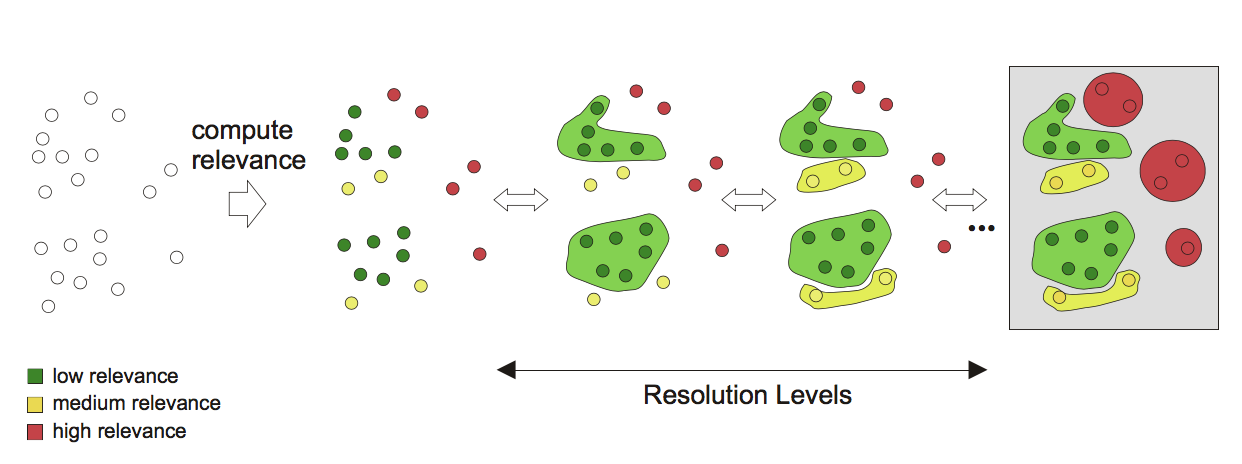
\includegraphics{src/images/multi-resolution}}
     \caption{\textit{Multi-Resolution: }data items are grouped with variying granularity depending on their relevance. From  \cite{Keim2005}}
     \label{multi-resolution}
 \end{figure}
 In a multi-resolution visualization the resolution is usually less granular at the \textit{Overview-Level} and more granular at the \textit{Detail-Level}. \textit{CircleView} is one visualization technique with a multi-resolution metaphor. Multi-resolution is one important aspect for visualization tools to improve visual scalability.\\*
\textbf{Aggregation Markers:}\label{aggregationmarkers} A different approach for advanced visual metaphors are aggregation markers which were already mentioned by Shneiderman  \cite{Shneiderman2008}. He proposed to extend the Information Seeking Mantra  \cite{Shneiderman1996} with point clustering which he called aggregation markers. Point clustering groups a larger set of data points onto a smaller set in the 2D-plane  \cite{Morrison2014}. This process decreases the visual overlap of data points and thus, increases the perception of large data sets. Moreover, point clustering accelerates the rendering process by first rendering the data clusters  and later loading more detailed data items. This incremental loading fulfills user satisfaction by shorter response times.\\*
In contrast to data reduction methods advanced visual metaphors are not actually decreasing data size. They only decrease the \textit{perceived data volume} and keep the actual data volume. This differentiates methods like multi-resolution and aggregation markers from methods like data reduction. 


\section{Interaction Techniques}
Interaction Techniques describe how the user can interact with the data. In this section interaction techniques for large data sets are discussed and how they can enhance scalability. As discussed in \ref{problems} challenges in visualization are pixel overlap, limited screen space, identifying a region of interest and navigation. Interaction technique can overcome these problems. 
\par
Overlap can be eliminated by filtering and zooming as filters and zoom reduce the displayed data and hence, minimize the overlap. \\*
\textbf{Filtering:} With filters a set of variables can be selected and the visualization is only showing the respecting variables. The excluded data items are kept in memory.
One way of filtering are dynamic queries. They provide a filter-mechanism by multiple widgets, such as sliders or input fields  \cite{Hochheiser2004,Shneiderman2008,Aigner2011}. A specific dynamic query for time-oriented data are time-boxes. These boxes are rectangular selection areas which are drawn by the user. The tool then only displays values with a similar pattern to the pattern in the time-boxes.\\*
\textbf{Zooming} is the way of drilling down into a data set to a lower level of detail. The user focus is shifted from the \textit{Overview}-Level to a \textit{Detail-Level} where the displayed data is reduced and thus, overlap decreased. One special way of zooming is semantic zooming  \cite{Boulos2003}. Instead of zooming multiple linked views are preferred for a higher number of displayed object. This will be discussed in \ref{zoomingVsmultiple}. 
\par

The limited screen space can be enhanced by \textit{interactive distortion techniques} \cite{Mackinlay1991}.
The main idea of distortion techniques is to present more relevant data enlarged in the user focus while less relevant data are shown at the context in a smaller presentation. Distortion technique are not providing additional pixel to the existing screen pixels but they enhance the screen space metaphor by prioritizing screen pixels.
Examples for distortion techniques are \textit{Bifocal Displays}  \cite{Spence1982}, \textit{Fish-eye Views} and \textit{Perspective walls \cite{Keim2005},  \cite{Mackinlay1991}}.\\*
All distortion techniques transform the undistorted 2D space by a mathematical function and bring more relevant data points to the focus.\\* 
\textbf{Bifocal Displays} (figure \ref{fig:bifocal}) bend the space with a linear function.\\*
\textbf{Fish-eye Views} (figure \ref{fig:fisheye}) (also known as Table and Magnification Lense) apply a power function and\\*
\textbf{Perspective walls} (figure \ref{fig:perspectivewall}) distort the space by applying both linear and power function. Thus, a 3D-representation is created which exists of three walls. The front wall shows details and the two side walls provide context. Perspective walls is one method to provide \textbf{Focus + Context} and Navigation in large data sets.
\begin{figure}[H]
    \centering
        \scalebox{.25}{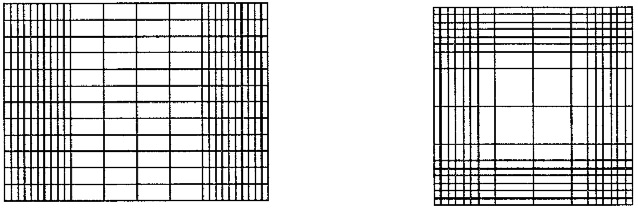
\includegraphics{src/images/f06b}}
    \caption{Bifocal Displays: distortion by linear function. From  \cite{Stroe1999}.}
    \label{fig:bifocal}
\end{figure}

\begin{figure}[H]
    \centering
        \scalebox{.25}{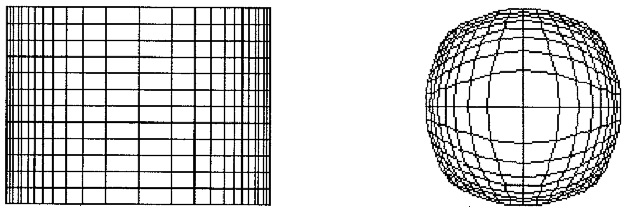
\includegraphics{src/images/f11c}}
    \caption{Fish-eye views:  distortion by a power function with an odd exponent  \cite{Stroe1999}.}
    \label{fig:fisheye}
\end{figure}

\begin{figure}[H]
    \centering
        \scalebox{.25}{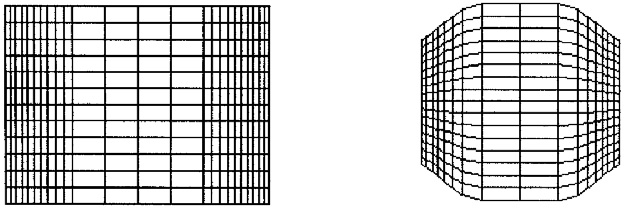
\includegraphics{src/images/f10b}}
    \caption{Perspective Walls: distortion by a half linear and half power function From  \cite{Stroe1999}.}
    \label{fig:perspectivewall}
\end{figure}
Distortion techniques are good in finding outliers. One disadvantage is that the user might loose the context.
\par

\label{navigation}
In close relation to interaction techniques stand appropriate \textit{interactive navigation techniques} to navigate inside the data set such as linked views and information murals, also known as navigational maps  \cite{Jerding1998}. With linked views the user can see different level of detail on one glance and navigate in different level of detail with navigational maps. Navigation also helps in finding a region of interest.\\*. The differentiation between navigation and interaction techniques is not selective.
\label{zoomingVsmultiple}
Ware  \cite{Ware2012} showed in figure \ref{fig:zoomVsMultiWindow} that zooming is an easy-to-use-tool for a small amount of items. However, if the user needs to keep three items or more in its visual working memory multiple windows are more effective than zooming. Thus, displaying large time-oriented data requires a layout with multiple simultaneous views if the number of data objects exceeds three items. Multiple coordinated views are called linked views. Often, linked views are combined with Brushing. \\*

\textbf{Brushing \& Linking: }The user can select data items on the screen(Brushing) and the respective items are highlighted in every connected window (Linking) which is also known as coordinated window. Therefore, lasso, rubber-band or rectangular selection enables the user to select groups of data items  \cite{Tegarden1999, Aigner2011}. Brushing \& Linking is one way to achieve \textit{Focus + Context} but it also supports the user by the user task \textbf{T3} as similar items are highlighted. Moreover, in the context of time-oriented data a typical brushing activity is the selection of an smaller time-span to see more details during this period of time. 
\\*

\begin{figure}[H]
    \centering
        \scalebox{.3}{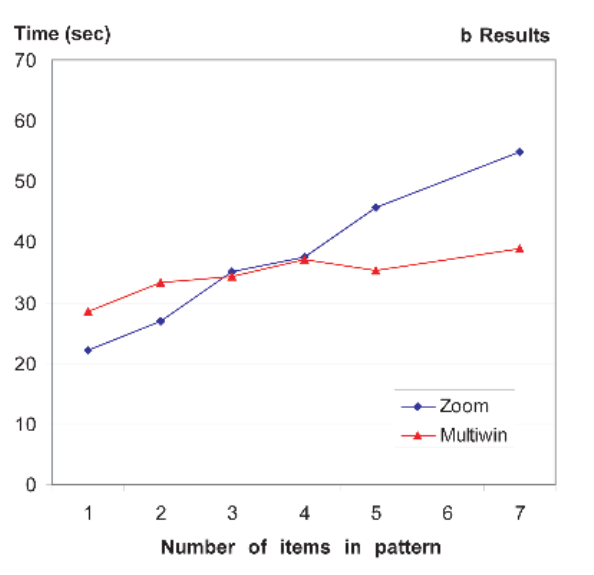
\includegraphics{src/images/zoomVSmultiWindow}}
    \caption{Measured task performance of zooming compared to multiple windows.  \cite{Ware2012a}}
    \label{fig:zoomVsMultiWindow}
\end{figure}

Another navigation technique for large data sets are \textbf{navigational maps}.\\*
\textbf{Navigational Maps: } display the complete data set next to other linked views as a miniature version in a separate window. With this method, the user can as well see the data set in detail as well keep the context and navigate through the data set.\\*
\textbf{Search: }\label{search} Besides navigational maps \textit{Searching} is an approach in querying and retrieving one specific data point. Searching uses natural language processing (NLP). As data set searching can include solutions from the text input at the front-end or it also can consider solutions from the data points - displayed in the visualization. The second case is recommended for large data as the number of data points is difficult to overview.
\par

The discussed interaction techniques are only a subset of available interaction techniques. We focused on interaction styles which can solve the problems of large data visualization and thus enhance visual scalability  \cite{Tegarden1999}. Hereby, we assume that interaction is in responsibility of the visualization tools.


\begin{table}[H]

    \begin{tabular}{|l| l l l|}
        \hline
            &                   & 1 & 2\\
        \hline
            &                   & \begin{turn}{90} Multi-Resolution\end{turn}   & \begin{turn}{90} Aggregation\end{turn}\\
        \hline
        A   & avoids overlap    & \checkmark                                    &\\
        B   & keeps spatial information     & x                                 &\\
        C   & can be localised  & \checkmark                                    &\\
        D   & is scalable       & \checkmark                                    &\\
        E   & is adjustable     & x                                             &\\
        F   & can show point/ line attribute    & x                             &\\
        G   & can discriminate points/ lines    & x                             &\\
        H   & can see overlap density           & x                             &\\
        \hline
    \end{tabular}
\end{table}



\section{Success Criteria for large scale data visualization}\label{success}
After our analysis of the limiting factors for displaying large data sets we come to the conclusion that the limitation by human perception is more restrictive than the limitation by different visualization techniques. The question is \textit{not} how many pixel can be displayed by a visualization technique but whether the visualization technique allows to perceive patterns. This is achieved by the use of \textit{appropriate visual metaphors} and \textit{data reduction methods}. Data reduction methods can aggregate overlapping data items to cluster by either mapping data density to color or by displaying the mean and the range of data. Visual Metaphors include techniques such as multi-resolution and thus, enhance the number of pixels which can be displayed. Data and dimension reduction reduces the number of data items which needs to be displayed. Thus, even non-scalable visualization techniques can display the reduced data. 
\par

Bringing all findings together, the important factors for the visualization of large data sets to support decision-making are the following: 
\begin{enumerate}[noitemsep]
\item How are advanced visualization techniques integrated? 
\item How is data reduction achieved? 
\item How are aggregation metaphors implemented? 
\item How are interaction techniques supported?
\end{enumerate}

Visualization tools need to offer solutions to these questions for a successful visualization of large data sets. Thus, we propose the following success criteria for large data visualizations and define a best possible implementation. This definition will be equivalent to the best score for completeness of the scoring model in chapter \ref{chap:Tools}.
\begin{enumerate} [noitemsep]
\item Analytical Techniques 
\begin{enumerate}
    \item The tool offers horizontal data reduction.
    \begin{itemize}
        \item Let $k$ be the desired number of dimensions. A data set can be reduced to $k$ dimensions. The visualization takes $k$ dimensions as input.
        \item Dimensions can be aggregated and saved as a new dimension.
    \end{itemize}
    \item The tool offers vertical data reduction.
    \begin{itemize}
        \item Data sets can be reduced by omitting rows.
        \item Filter are offered to interactively reduce the number of showed data items.
        \item Data points can be removed from data set. 
        \item Relevance can be assigned to data points so that important data points can be kept and less relevant data points removed.
        \item Data items can be clustered and saved.  
    \end{itemize}
\end{enumerate}


\item Visualization Techniques
\begin{enumerate}
\item The tool offers all possible visualization techniques.
\item Every visualization technique can cluster or aggregate data items.
\item Every visualization technique can use multi-resolution.
\end{enumerate}

\item Interaction Techniques
\begin{enumerate}
\item The tool offers the drill-down functions zoom and filter for every visualization.
\item The tool offers the distortion techniques fish-eye, perspective wall, bifocal display for every visualization.
\item The tool offers the navigation techniques navigational maps, coordinated windows, searching for every visualization.
\end{enumerate}

\end{enumerate}

In the next chapter we will compare different state-of-the art tools regarding this success criteria for large data visualization.
